% =====================================================================
%  Chapitre 1 -- Du MLP aux CNN
%  Partie b : le mur du MLP, en chiffres
% =====================================================================

\begin{frame}{La question du coût : combien de paramètres ?}
\begin{columns}[t]
\begin{column}{0.50\textwidth}
\begin{itemize}
  \item Un neurone d'une couche dense connectée à $n$ entrées porte $n$ poids
  \textbf{plus un biais}.
  \item Une couche dense à $n$ entrées et $m$ neurones coûte donc
  $n \times m + m$ paramètres.
  \item Sur une image, $n$ est le nombre de \textbf{pixels}, pas le nombre
  d'objets : il croît comme le carré de la résolution.
\end{itemize}
\begin{kbox}[La règle du coût]
$\text{paramètres} = n_{\text{entrées}} \times n_{\text{neurones}} + n_{\text{neurones}}$

\medskip
Toute la suite découle de cette seule formule.
\end{kbox}
\end{column}
\begin{column}{0.46\textwidth}
\centering
\end{column}
\end{columns}
% [fix] figure sortie
\end{frame}

\begin{frame}{La question du coût : combien de paramètres ? --- la figure}\begin{center}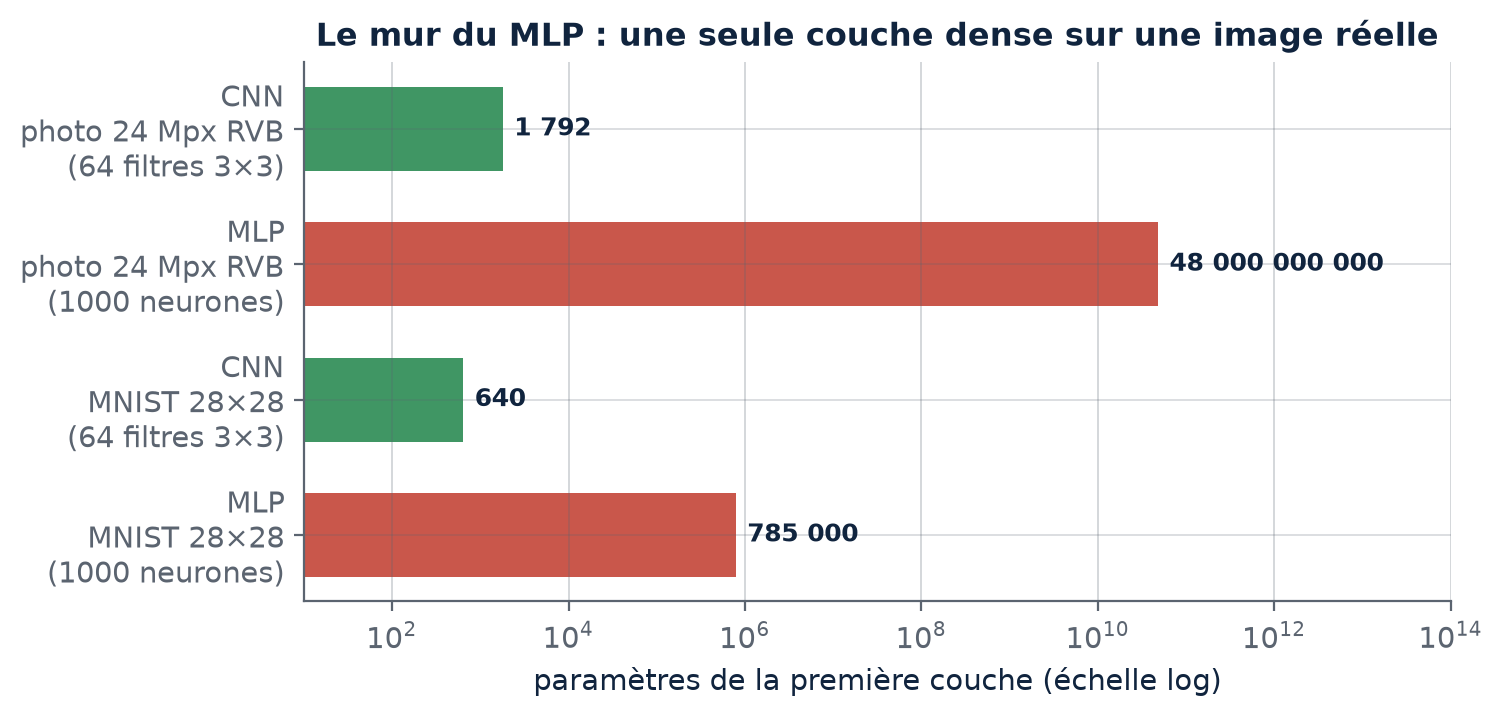
\includegraphics[width=.92\textwidth]{f01_mur_du_mlp.png}\end{center}\end{frame}

\begin{frame}[fragile]{Calcul 1 --- le cas MNIST, qui passe encore}
\begin{columns}[t]
\begin{column}{0.52\textwidth}
\begin{itemize}
  \item MNIST : images de $28 \times 28$ pixels, donc
  $28 \times 28 = 784$ entrées après aplatissement.
  \item Une première couche dense de $1\,000$ neurones :
  \[
  784 \times 1\,000 + 1\,000 = 784\,000 \text{ paramètres}
  \]
  \item Le réseau entier atteint quelques millions de paramètres : c'est
  \textbf{encore gérable} sur un ordinateur portable.
\end{itemize}
\begin{wbox}[Mais le principe est déjà mauvais]
784\,000 paramètres pour lire un chiffre de $28 \times 28$ : chacun est
connecté à \emph{tous} les pixels, y compris ceux de l'angle opposé.
\end{wbox}
\end{column}
\begin{column}{0.44\textwidth}
\begin{codebox}[Le calcul, en Python]
\begin{lstlisting}
cote = 28
entrees = cote * cote      # 784
neurones = 1000
p = entrees * neurones + neurones
print(p)                   # 784000
\end{lstlisting}
\end{codebox}
\begin{solbox}[Vérification]
$784 \times 1\,000 = 784\,000$, plus $1\,000$ biais :
le total est bien $784\,000$.
\end{solbox}
\end{column}
\end{columns}
\end{frame}

\begin{frame}[fragile]{Calcul 2 --- une vraie photo : le mur}
\begin{columns}[t]
\begin{column}{0.52\textwidth}
\begin{itemize}
  \item Une photo d'appareil moderne : environ $4\,000 \times 4\,000$ pixels,
  en couleur (3 canaux).
  \item Nombre d'entrées après aplatissement :
  \[
  4\,000 \times 4\,000 \times 3 = 48\,000\,000
  \]
  \item La même couche dense de $1\,000$ neurones :
  \[
  48\,000\,000 \times 1\,000 \approx 48 \text{ milliards de paramètres}
  \]
  \item C'est \textbf{mort} : ni la mémoire, ni les données, ni le temps
  d'entraînement ne suivent.
\end{itemize}
\end{column}
\begin{column}{0.44\textwidth}
\begin{codebox}[Le calcul, en Python]
\begin{lstlisting}
cote = 4000
canaux = 3
entrees = cote*cote*canaux
print(entrees)        # 48000000

p = entrees*1000 + 1000
print(p)              # 48001000000
\end{lstlisting}
\end{codebox}
\begin{wbox}[48 milliards de paramètres]
pour classer \emph{une seule} image de 24 mégapixels. Aucun jeu de données
ne peut entraîner autant de poids.
\end{wbox}
\end{column}
\end{columns}
\end{frame}

\begin{frame}{Le CNN sur la même photo : 1 792 paramètres}
\begin{columns}[t]
\begin{column}{0.52\textwidth}
\begin{itemize}
  \item Un noyau $3 \times 3$ appliqué à une entrée à 3 canaux contient
  $3 \times 3 \times 3 = 27$ poids.
  \item Avec $64$ filtres de ce type et $64$ biais :
  \[
  3 \times 3 \times 3 \times 64 + 64 = 1\,792 \text{ paramètres}
  \]
  \item Rapport avec la couche dense :
  \[
  \frac{48\,010\,000\,000}{1\,792} \approx 26\,781
  \]
\end{itemize}
\begin{kbox}[Pourquoi une telle différence ?]
Le noyau \textbf{ne connaît pas la taille de l'image} : ses $27$ poids sont
réutilisés à chaque position. La couche dense, elle, apprend un poids
\emph{par pixel}.
\end{kbox}
\end{column}
\begin{column}{0.44\textwidth}
\begin{center}
\begin{tabular}{@{}lr@{}}
\toprule
\textbf{Couche} & \textbf{Paramètres} \\
\midrule
dense, 48 M entrées & 48\,010\,000\,000 \\
conv 3$\times$3, 64 filtres & 1\,792 \\
\midrule
\textbf{ratio} & $\approx 26\,781\times$ \\
\bottomrule
\end{tabular}
\end{center}

\end{column}
\end{columns}
% [fix] bloc deplace
\end{frame}
\begin{frame}{Le CNN sur la même photo : 1 792 paramètres (suite)}
\begin{solbox}[Même image, même tâche, deux ordres de grandeur]
Le partage de poids n'est pas une optimisation : c'est ce qui rend le
problème \emph{apprenable}.
\end{solbox}
\end{frame}

\begin{frame}{Activité 1 --- estimer un coût avant de coder}
\begin{abox}[À vous de jouer (10 min)]
Calculez, à la main puis vérifiez avec Python :
\begin{enumerate}
  \item Une couche dense sur une entrée $224 \times 224 \times 3$ vers
  $1\,000$ neurones.
  \item Une couche convolutive $3 \times 3$, $64$ filtres, sur la même entrée.
  \item Le rapport entre les deux.
\end{enumerate}
\end{abox}
\begin{solbox}[Correction]
\begin{itemize}
  \item Dense : $224 \times 224 \times 3 = 150\,528$ entrées, soit
  $150\,528 \times 1\,000 + 1\,000 = 150\,529\,000$ paramètres
  ($\approx 150$ millions).
  \item Conv $3 \times 3$ : $3 \times 3 \times 3 \times 64 + 64 = 1\,792$ paramètres.
  \item Rapport : $\approx 84\,000\times$.
\end{itemize}
\medskip
\textbf{Leçon :} même sur une image « petite » de 224 pixels, la couche dense
est déjà hors de portée.
\end{solbox}
\end{frame}

\begin{frame}{Quiz 1 --- le coût des paramètres}
\begin{qbox}[Question 1]
Une entrée de $64 \times 64$ en niveaux de gris vers une couche dense de
$500$ neurones coûte :
\begin{itemize}
  \item[(a)] $32\,000$ \quad (b) $32\,500$ \quad (c) $4\,096 \times 500$ paramètres
\end{itemize}
\end{qbox}
\begin{qbox}[Question 2]
Pourquoi le nombre de paramètres d'une couche convolutive ne dépend-il pas
de la taille de l'image ?
\begin{itemize}
  \item[(a)] Parce que le noyau est petit \quad (b) Parce que les poids sont
  partagés entre toutes les positions \quad (c) Parce que le pooling réduit l'image
\end{itemize}
\end{qbox}
\begin{qbox}[Question 3]
On double la résolution d'une image ($cote \to 2 \times cote$). Le coût de la
couche dense :
\begin{itemize}
  \item[(a)] double \quad (b) est multiplié par 4 \quad (c) est multiplié par 8
\end{itemize}
\end{qbox}

% [fix] bloc deplace
\end{frame}
\begin{frame}{Quiz 1 --- le coût des paramètres (suite)}
\begin{solbox}[Réponses]
\textbf{1.} (b) : $64 \times 64 = 4\,096$ entrées, $4\,096 \times 500 + 500 = 2\,048\,500$ ;
l'option (a) oublie les biais, la (c) aussi. \quad
\textbf{2.} (b) : le même noyau est appliqué partout. \quad
\textbf{3.} (b) : le nombre de pixels croît comme le \emph{carré} de la résolution.
\end{solbox}
\end{frame}
